\section{OptSQL}
\label{sec:OptSQL}

\subsection{Overview}
Figure~\ref{fig:overview} shows the overall architecture of \toolname.
Given a NL question and a database environment, \toolname\ aims to generate a SQL query that is both semantically correct and execution-efficient.
Instead of treating Text-to-SQL as a fixed pipeline, \toolname\ formulates it as a feedback-driven process coordinated by a Meta-Cognitive Controller.
%
The Meta-Cognitive Controller supervises the entire workflow.
It perceives the database environment, estimates the difficulty of the input question, selects suitable actions, and monitors intermediate feedback throughout both generation and optimization.
Under its control, \toolname\ first constructs an initial SQL query in the Generation Phase, where an evidence-guided schema filter identifies relevant tables, columns, values, and join paths, and an initial SQL builder produces executable candidate queries.
If the controller detects that the query requires further efficiency improvement, it activates the Optimization Loop.
This loop consists of an Explain Analyzer Agent, a SQL Rewriter Agent, and a Validator Agent, which together analyze execution plans, rewrite inefficient SQL patterns, and verify semantic consistency and cost reduction.
%
\toolname\ is further supported by a Memory Engine and a Tool Infrastructure.
The Memory Engine maintains both task-level working memory and reusable optimization knowledge, including expert rules, historical rewrite cases, and observed optimization patterns.
The Tool Infrastructure provides database grounding, SQL execution and analysis, cost evaluation, semantic consistency checking, and RAG-based retrieval.
Through these components, \toolname\ continuously observes feedback from the database environment, reflects on its intermediate decisions, and updates its optimization experience.

\begin{figure*}[t]
	\centering
	%	\vspace{-3mm}
	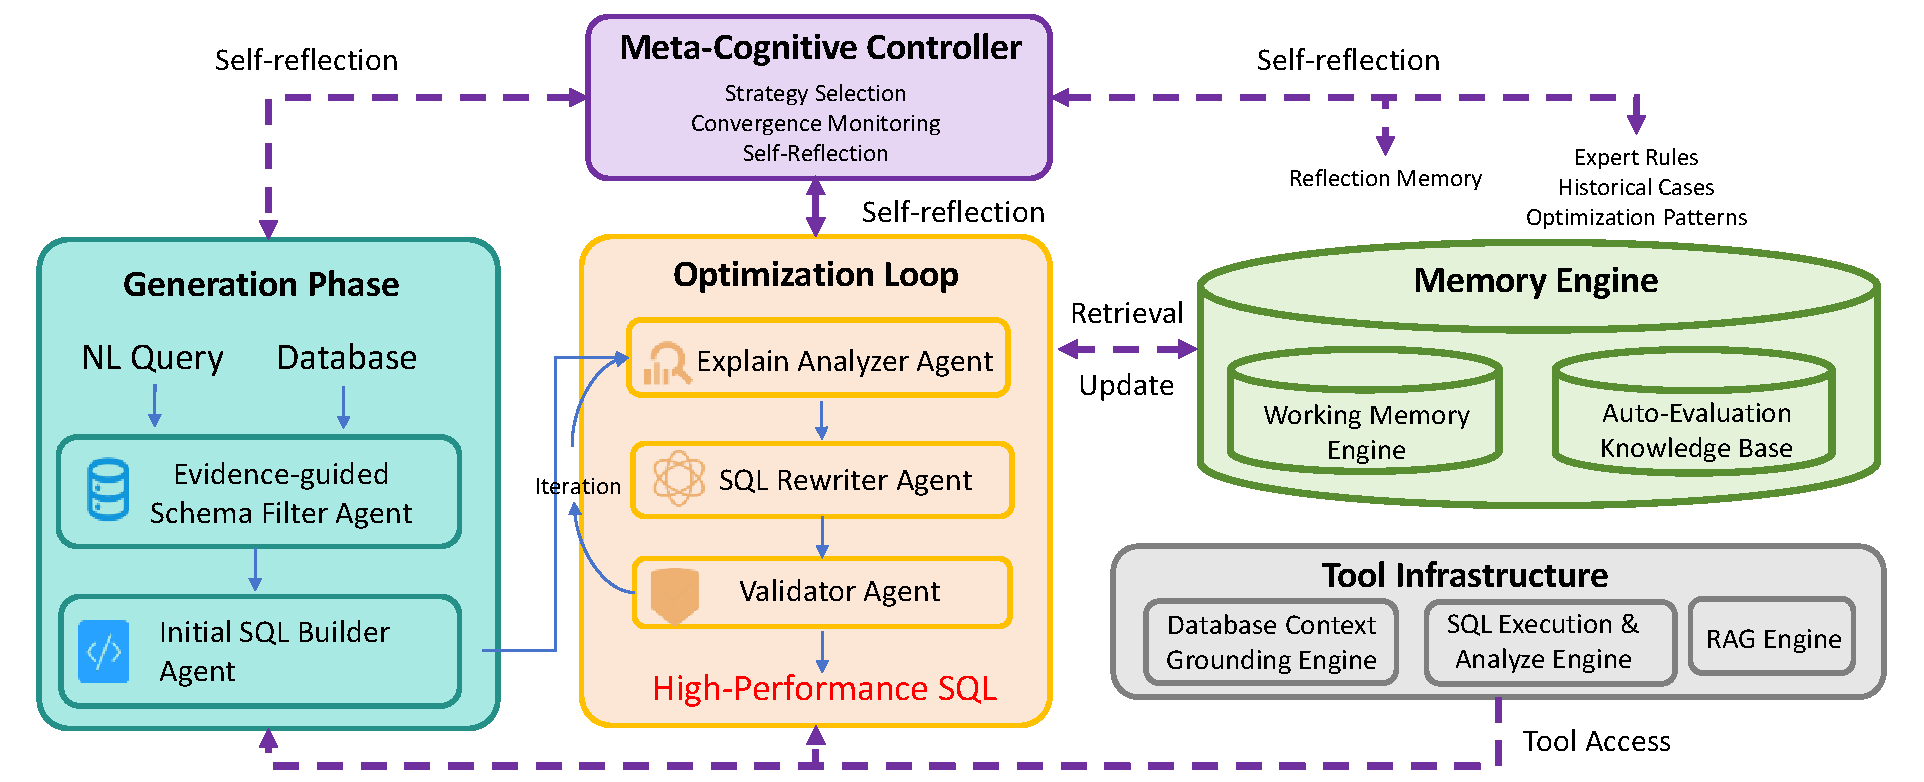
\includegraphics[width=1\linewidth]{./images/overview.pdf} 
	\vspace{-5mm}
	\caption{\textbf{Overview of \toolname}}
	\label{fig:overview}
	\vspace{-4mm}
\end{figure*}

The remainder of this section describes each component of \toolname.
We first present the Generation Phase for constructing an initial SQL query (Section~\ref{subsec: Generation Phase}), followed by the Optimization Loop for execution-aware rewriting (Section~\ref{subsec: Optimization Loop}).
We then introduce the Meta-Cognitive Controller that orchestrates these processes through strategy selection, monitoring, and self-reflection (Section~\ref{subsec: Meta-Cognitive Controller}).
Finally, we describe the Memory Engine and Tool Infrastructure that support retrieval, experience accumulation, and database feedback (Section~\ref{subsec: Memory Engine and Tool Infrastructure}).

\subsection{Generation Phase}
\label{subsec: Generation Phase}
The Generation Phase aims to construct a set of executable and semantically plausible initial SQL candidates based on the question and database environment.
It focuses on two core capabilities: evidence construction and multi-strategy SQL generation, without global control or optimization decisions.

\textbf{Evidence-guided Schema Filter Agent.}
This agent is responsible for grounding the input question into a compact, relevant, and executable schema context for downstream SQL generation.
This agent is responsible for grounding the input question into a compact, relevant, and executable schema context for downstream SQL generation.
It combines robust schema linking with value-level grounding, aiming to identify not only the tables and columns mentioned or implied by the question, but also the concrete database values and conditions needed to express the user intent.
To improve schema robustness, the agent supports multiple complementary schema linking strategies:

\begin{itemize}[leftmargin=10pt]
	\item \textit{Direct schema linking} maps the natural language question to relevant tables and columns by reasoning over question semantics and schema descriptions.
	This strategy is effective when the question contains explicit lexical or semantic cues.
	
	\item \textit{Reverse schema linking} hypothesizes a tentative SQL structure and then extracts the tables and columns implied by this structure~\cite{li2026deepeye}.
	This recovers latent schema dependencies, such as join tables, grouping columns, or aggregation-related attributes, that may be missed by direct matching.
	
	\item \textit{Value-grounded schema linking} identifies relevant schema elements through actual database contents.
	Instead of relying only on table or column names, the agent checks whether values in a column match or semantically correspond to phrases in the question, which is especially useful when schema names are ambiguous or weakly informative.
\end{itemize}

Beyond schema linking, the agent further performs active value grounding to translate natural language expressions into concrete database predicates.
It supports several value grounding capabilities:

\begin{itemize}[leftmargin=10pt]
	\item \textit{Exact value verification} checks whether a phrase in the question directly appears in candidate columns.
	This is useful for grounding categorical conditions such as names, locations, statuses, or labels.
	
	\item \textit{Semantic value matching} retrieves column values that are semantically close to question phrases, allowing the agent to handle paraphrases, abbreviations, and domain-specific expressions.
	
	\item \textit{Distinct-value inspection} examines representative or unique values of a column to infer how natural language concepts are encoded in the database, such as whether a Boolean concept is represented by \texttt{0}/\texttt{1}, \texttt{Y}/\texttt{N}, or textual labels.
	
	\item \textit{Data sampling and distribution checking} inspects example rows or value distributions to understand column semantics and avoid grounding predicates on irrelevant or sparsely populated columns.
	
	\item \textit{Null and type analysis} checks whether candidate columns contain nulls or unexpected value formats, helping the agent avoid unreliable predicates and distinguish categorical, numerical, date, and Boolean constraints.
	
	\item \textit{Composite predicate grounding} combines multiple grounded values or columns when a natural language phrase corresponds to a compound condition, such as a grade span, date range, or multi-attribute status.
\end{itemize}

For example, a phrase such as ``kindergarten to 8th grade'' may be grounded as \texttt{Low\_Grade = 'K'} and \texttt{High\_Grade = '8'}, while ``magnet program'' may correspond to a binary or categorical value after inspecting the value distribution of a related column.
These grounded facts are passed to the SQL generator as explicit evidence, reducing the risk of hallucinated predicates or incorrect value choices.
Finally, the agent further completes the relational context required for SQL construction.
The selected schema elements may be semantically relevant but structurally disconnected; for example, two relevant tables may require intermediate tables or primary--foreign key columns to form a valid join path.
Therefore, the agent supplements necessary join keys and bridge tables according to the database relationships, so that the resulting schema context can support executable SQL generation.
The output of this agent is an evidence-enriched schema context that integrates schema relevance, verified value grounding, ambiguous-case evidence, and join-path information for downstream SQL generation.

\textbf{Initial SQL Builder Agent.}
Initial SQL Builder Agent is responsible for producing executable and semantically plausible initial SQL candidates.
It provides a set of complementary SQL construction capabilities, rather than a fixed generation pipeline.
Depending on the task complexity, schema ambiguity, and control signals from the Meta-Cognitive Controller, the agent may invoke one or more generation strategies to balance robustness and efficiency.
The agent supports the following SQL generation strategies:

\begin{itemize}[leftmargin=10pt]
	\item \textit{Skeleton-based generation} follows a top-down construction process.
	It first analyzes the required SQL components, such as selection, filtering, joining, grouping and ordering, then sketches a SQL skeleton, and finally fills in concrete tables, columns, predicates, and functions.
	This strategy is useful for queries that require clear structural planning.
	
	\item \textit{ICL-based generation} leverages retrieved demonstrations to guide SQL construction.
	By retrieving structurally similar examples, the agent can reuse successful query patterns and adapt them to the current grounded schema.
	This strategy is especially helpful when the question resembles previously observed SQL structures.
	
	\item \textit{Decomposition-based generation} breaks a complex question into simpler sub-questions and generates SQL fragments for each sub-task before composing them into a complete query.
	This strategy is designed for complex analytical questions involving nested reasoning, multiple conditions, or multi-step aggregation.
\end{itemize}

After candidate generation, the agent can apply a lightweight repair loop to improve executability.
It checks basic syntactic and execution errors, and revises invalid candidates using the original question, grounded schema evidence, and database error messages.
This repair process removes obvious generation failures before candidate selection, while leaving global strategy switching and deeper optimization to the Meta-Cognitive Controller.
When multiple candidates are available, the agent further supports \textit{execution-based selection}.
Candidates are grouped according to their execution results, and each group is treated as a behavioral cluster.
If one cluster forms a dominant majority, the agent selects a representative query from that cluster as the initial SQL.
Otherwise, representative candidates from the top clusters are compared through pairwise semantic judgment, and each candidate is ranked by a confidence-aware score.
%\[
%score(q) = conf(q) \times winRate(q).
%\]
The candidate with the highest score is selected as the output of the Initial SQL Builder Agent.


\subsection{Optimization Loop}
\label{subsec: Optimization Loop}

The Optimization Loop aims to improve the execution efficiency of an initial SQL query while preserving its semantics.
It is activated when the Meta-Cognitive Controller determines that the generated SQL may benefit from further optimization, such as when the query involves large tables, complex joins, or inefficient query plans.
Instead of treating SQL generation as the final step, this loop refines the initial query through execution-aware analysis, rewriting, and validation.

%\textbf{Explain Analyzer Agent.}
%This agent is responsible for diagnosing potential inefficiencies in the current SQL query.
%Given an initial SQL query, it inspects both the query structure and database feedback, including query plans, estimated costs, and observable bottleneck patterns.
%Based on this analysis, it produces optimization suggestions for the SQL Rewriter Agent.
%As shown in Table~\ref{tab:explain-analyzer}, the agent maintains a set of optimization patterns.
%Each pattern describes a possible inefficiency, a corresponding rewrite direction, and the safety condition under which the rewrite should be considered.
%These suggestions are not directly applied as deterministic rules.
%Instead, they serve as evidence for the SQL Rewriter Agent, which decides how to rewrite the query under semantic-preservation constraints.
%
%\begin{table*}[t]
%	\centering
%	\caption{\textbf{Optimization patterns used by the Explain Analyzer Agent.}}
%	\label{tab:explain-analyzer}
%	\small
%	\begin{tabular}{p{0.21\linewidth}p{0.34\linewidth}p{0.35\linewidth}}
%		\toprule
%		Pattern & Rewrite Direction & Safety Condition \\
%		\midrule
%		Redundant projection
%		& Replace \texttt{SELECT *} with necessary projected columns.
%		& Applied when required output columns can be inferred from the question or generated SQL. \\
%		
%		Scalar \texttt{MAX}/\texttt{MIN} subquery
%		& Rewrite to \texttt{ORDER BY ... LIMIT 1}.
%		& Applied only when tie behavior and aggregation semantics are preserved. \\
%		
%		Correlated subquery
%		& Rewrite to \texttt{JOIN} or \texttt{CTE}.
%		& Applied when an equivalent rewrite pattern is retrieved or can be validated. \\
%		
%		Missing filter pushdown
%		& Move selective predicates closer to base tables.
%		& Applied when predicate movement does not change join or aggregation semantics. \\
%		
%		Late aggregation
%		& Pre-aggregate before join.
%		& Applied when grouping keys and aggregation semantics remain equivalent. \\
%		
%		Inefficient \texttt{OR} predicate
%		& Rewrite to \texttt{UNION} or \texttt{UNION ALL}.
%		& Applied when duplicate semantics are correctly handled. \\
%		
%		Redundant join path
%		& Simplify unnecessary joins or bridge tables.
%		& Applied only when projected columns and filtering semantics are unaffected. \\
%		
%		Function on indexed column
%		& Rewrite to an equivalent range or comparison predicate.
%		& Applied when the transformation preserves value semantics. \\
%		
%		Inefficient ordering
%		& Align \texttt{ORDER BY} / \texttt{LIMIT} with available ordering or indexes.
%		& Applied when ordering semantics are unchanged. \\
%		\bottomrule
%	\end{tabular}
%\end{table*}
%
%\textbf{SQL Rewriter Agent.}
%This agent transforms the current SQL query into a potentially more efficient variant.
%Its input includes the original SQL, optimization suggestions from the Explain Analyzer Agent, and optionally retrieved rewrite cases or expert rules from the Memory Engine.
%The rewriter is required to preserve the original query semantics while applying only the optimization actions supported by the available evidence.
%The rewriting process focuses on producing semantically equivalent SQL variants with lower estimated or actual execution cost.
%For example, it may remove unnecessary projections, push selective predicates closer to base tables, rewrite inefficient subqueries, avoid functions on indexed columns when an equivalent range predicate is available, or restructure joins and aggregations under explicit safety constraints.
%The output of this agent is a rewritten SQL query together with a brief explanation of the applied optimization rationale.
%
%\textbf{Validator Agent.}
%This agent verifies whether the rewritten SQL is both correct and beneficial.
%It performs two checks.
%First, it checks semantic consistency between the original SQL and the rewritten SQL, ensuring that the rewrite does not change the intended result.
%Second, it evaluates whether the rewritten SQL reduces execution cost, using estimated optimizer cost, execution latency, or other available database feedback.
%If the rewritten query violates semantic consistency, the result is rejected and returned for further reflection.
%If the rewritten query preserves semantics but fails to improve cost, the loop may either retry with a different rewriting strategy or terminate when no meaningful improvement is observed.
%Only when both semantic preservation and cost reduction are satisfied is the rewritten query accepted as the optimized output.
%
%Overall, the Optimization Loop provides an execution-aware refinement mechanism for \textsc{OptSQL}.
%The Explain Analyzer Agent identifies optimization opportunities, the SQL Rewriter Agent applies evidence-guided rewrites, and the Validator Agent ensures that the rewrite is both semantically safe and performance-improving.
%Through this loop, \textsc{OptSQL} can transform an initially correct SQL query into a higher-performance query under the supervision of the Meta-Cognitive Controller.

\subsection{Meta-Cognitive Controller}
\label{subsec: Meta-Cognitive Controller}

\subsection{Memory Engine and Tool Infrastructure}
\label{subsec: Memory Engine and Tool Infrastructure}








